\documentclass{article}
\usepackage[utf8]{inputenc}
\usepackage{fullpage}
\usepackage{amsmath}
\usepackage{hyperref}
\usepackage{amssymb}
\usepackage[most]{tcolorbox}
\usepackage{empheq}
\usepackage{mhchem}
\usepackage{braket}
\usepackage{graphicx}
\usepackage{subcaption}

\newtcbox{\mymath}[1][]{%
    nobeforeafter, math upper, tcbox raise base,
    enhanced, colframe=black!30!black,
    colback=black!30, boxrule=1pt,
    #1}
    
\title{Computational Physics HW 3}
\author{Marcus DuPont}
\date{\today}

\begin{document}

\maketitle

\begin{enumerate}
    \item {\textbf{Newman 7.2}
    \begin{enumerate}
        \item{From looking at the plot, I estimate a period of roughly 140 months per cycle.
        \begin{figure}[htp]
            \centering
            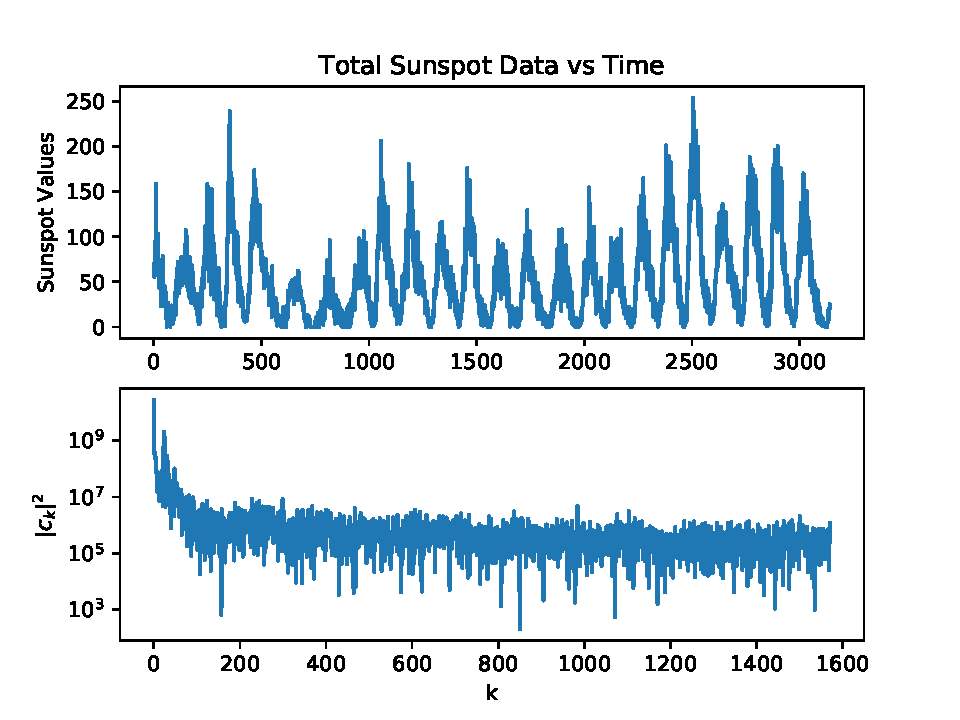
\includegraphics[width=\textwidth]{sunny.pdf}
            \caption{Sunspot Data vs Time in the top panel and the power spectrum of the solar cycle is shown in the bottom panel. We see the power spectrum peak at about 24/month.}
            \label{fig:my_label}
        \end{figure}
        }
        \item{The period is given by:
        \begin{equation*}
            \tau = \frac{2\pi}{\omega} = \frac{2\pi}{2\pi k/N} = \frac{N}{k}
        \end{equation*}
        Using this formula, we arrive at the following output:
        \begin{quote}
            \$ ./sunspot.py \\
            Performing DFT...\\
            The maximum occurs at a frequency: 24/month\\

            This corresponds to a period of 130.95833333333334 months
        \end{quote}}
    \end{enumerate}
    }
    \item {\textbf{Newman 7.9}
    \begin{enumerate}
        \item{The results are shown Figure (2):
        
        
        \begin{figure}
            \centering
            \begin{subfigure}[b]{0.5\textwidth}
                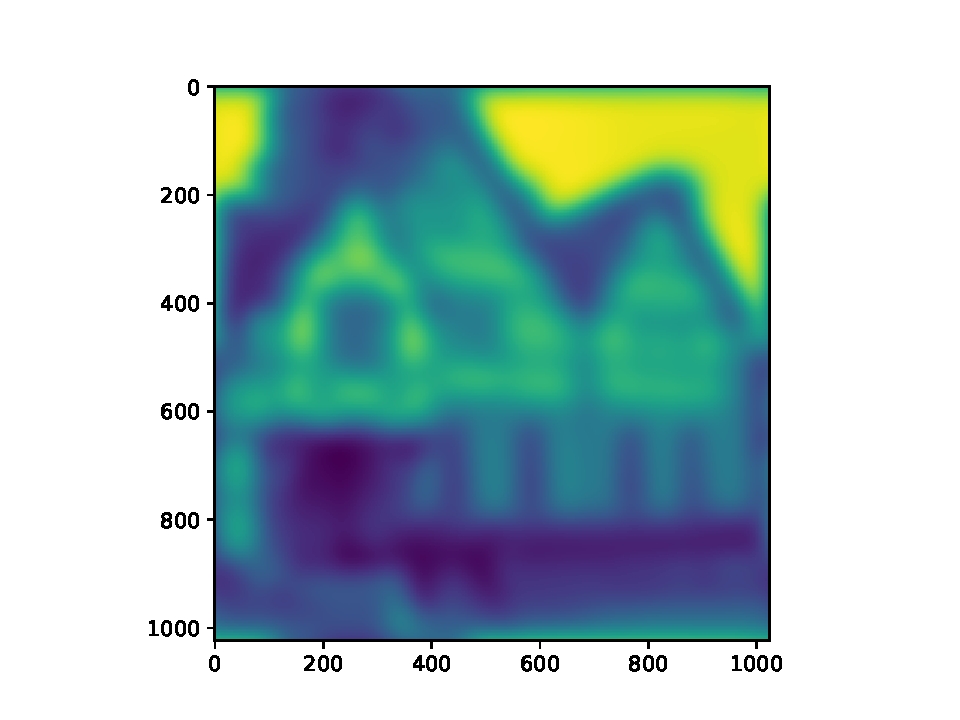
\includegraphics[width=\textwidth]{blurred_photo.pdf}
                \caption{The blurred image that is given by the raw data}
                \label{fig:gull}
            \end{subfigure}
            ~ %add desired spacing between images, e. g. ~, \quad, \qquad, \hfill etc. 
              %(or a blank line to force the subfigure onto a new line)
            \begin{subfigure}[b]{0.5\textwidth}
                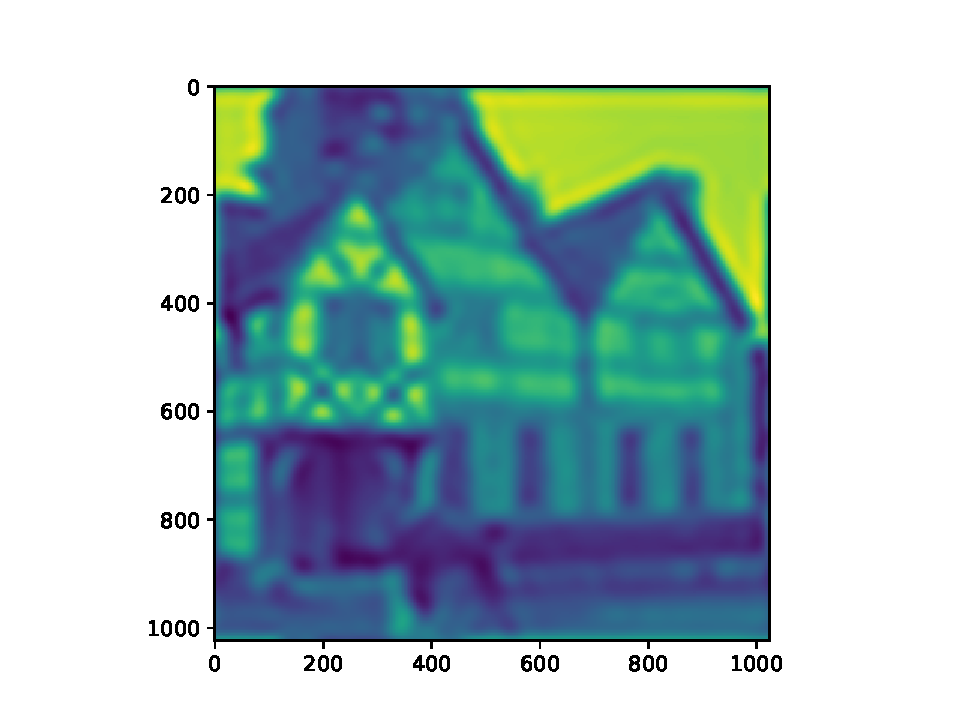
\includegraphics[width=\textwidth]{unblurred.pdf}
                \caption{The ``unblurred'' image after performing the necessary Fourier transform to the $\Tilde{a_k}$ coefficients.}
                \label{fig:tiger}
            \end{subfigure}
            ~ %add desired spacing between images, e. g. ~, \quad, \qquad, \hfill etc. 
            %(or a blank line to force the subfigure onto a new line)
        \end{figure}
        
        }
        \item{Why can't we make photos completely sharp?\\
        
        \textbf{Answer:}\\
        With images, there is information that is stored within them. When we work to manipulate these images, there is potential for bits of information to be lost as we perform the necessary transformations to unblur the images. Furthermore, in order to completely unblur images, there is also the requirement of having the ``perfect'' PSF for said images, which isn't realistic.}
    \end{enumerate}
    }
\end{enumerate}

\end{document}
